\documentclass[11pt]{scrartcl}
\usepackage[utf8]{inputenc}
\usepackage{evank}


%% insert title here
\newcommand{\titlee}{Induction [Solutions]}
\parindent 0 pt

\newcommand{\officialsol}[1]{See the official solutions \href{#1}{here}.}

\title{\titlee}
\author{Cambridge Physics Academy}
\date{2023-2024}


\begin{document}

\thispagestyle{empty}
\begin{center}
    
    
    \Huge \textbf{\textsf{\titlee}}

    \large \theauthor
\end{center}

\setcounter{section}{-1}
\section{Readings}
\begin{itemize}
    \item Ch 34-36 of HRK
    \item Ch 7 of Purcell
\end{itemize}
Feel free to do problems from the readings as extra practice.


\section{Lecture review}

\begin{defn}[Electromotive Force]
    The electromotive force, denoted by $\mathcal E$ is a generalization of the potential difference. Instead of just looking at the the electric field, it looks at the force per charge from the lorentz force:
    $$\mathcal E = \int ((\mathbf v \times \mathbf B) + \mathbf E )\cdot d\mathbf r.$$
\end{defn}
For a fixed loop moving in a temporally constant magnetic field (not necessarily spatially), integrating the expression above (check this as an exercise for yourself!) gives,
$$\mathcal E = \int (\mathbf v \times \mathbf B) \cdot d\mathbf r = -\frac{d\Phi_B}{dt}.$$
More generally, for a non-temporally constant magnetic field, we have Faraday's law.

\begin{theorem}[Faraday's Law]
    In the case of a changing magnetic field and/or a loop moving in a non-uniform magnetic field, the emf induced in the loop is given by
    $$\mathcal E = -\frac{d\Phi_B}{dt} \iff \oint \mathbf E \cdot d\mathbf r = -\frac{d\Phi_B}{dt}.$$
The negative sign in Faraday's Law above indicates \highlight{Lenz's Law}: the emf induced in a loop of wire is such that the generated magnetic field opposes the change in the external magnetic flux.
\end{theorem}

\begin{defn}[Self-Inductance]
    A circuit element can \textit{induce} a current within itself through its self-generated magnetic field. This is characterized by the inductance, which is defined as
    $$\Phi_B = LI, V = -\frac{d\Phi_B}{dt}  =-L\frac{dI}{dt}.$$
    The energy stored within an inductor is given by
    $$U = \frac 12 LI^2.$$
\end{defn}

\begin{defn}[Mutual Inductance]
    If you have two inductors of inductance $L_1,L_2$, then the total magnetic flux through each is given by
    \begin{align*}
    \Phi_1 &= L_1I_1 +M_{12}I_2,\\
        \Phi_2 &= L_2 I_2 + M_{21}I_1.
\end{align*}
\end{defn}

\begin{theorem}
    The mutual inductances are always equal,
    $$M_{12} = M_{21}.$$
\end{theorem}

\begin{idea}[LR Circuits]
    If you connect a inductor with constant current to a resistor in series, its current will decay exponentially,
    $$I(t) = I_0 e^{-t/\tau} , \tau = L/R,$$
    where $\tau$ is the time constant. Intuitively, the inductor always wants to keep the same amount of current flowing through it.
\end{idea}


\section{Problem Set}

\subsection{Exercises}


\begin{prob}
    In class we determined the effective inductance of two inductors where we assumed the mutual inductance was negligible. This time, assume that the mutual inductance between the two inductors with inductances $L_1$ and $L_2$ is a non-negligible value $M = M_{12} = M_{21}$, and find the total effective inductance when
    \begin{anum}
        \item They are connected in series.
        \item They are connected in parallel.
    \end{anum}
\end{prob}

\begin{alphasol}
    \item In series we have that the same current flows through them. Thus, the potential drop across ecah of them is
    $$V_1 = -L_1\frac{dI}{dt} - M \frac{dI}{dt}, V_2 = -L_2 \frac{dI}{dt} - M\frac{dI}{dt}.$$
    Thus, adding them together we get
    $$V_{\text{tot}} = -(L_1 + L_2 + 2M)\frac{dI}{dt},$$
    so the effective inductance is $L_{\text{eff}} = \boxed{L_1+L_2+2M}.$
    \item This one is a bit trickier. Let $I_1$ be the current through $L_1$ and $I_2$ be the current through $L_2$. Then, we have the following equations:
    \begin{align*}
        V &= -L_1\frac{dI_1}{dt} - M\frac{dI_2}{dt},\\
        V &= -L_2\frac{dI_2}{dt} - M\frac{dI_1}{dt}.
    \end{align*}
    Multiplying the first equation by $L_2 - M$ and the second by $L_1 -M$ we get
    \begin{align*}
        (L_2 - M) V &= -(L_1L_2 - ML_1)\frac{dI_1}{dt} - (L_2M - M^2) \frac{dI_2}{dt}.\\
        (L_1 - M) V &= -(L_1L_2 - ML_2) \frac{dI_2}{dt} - (L_1M - M^2)\frac{dI_1}{dt}.
    \end{align*}
    Adding the two now, we get
    $$(L_1 + L_2 - 2M) V = -(L_1L_2 - M^2)\frac{dI_1}{dt} - (L_1 L_2 - M^2)\frac{dI_2}{dt}.$$
    Thus, we can read off the effective inductance as $L_{\text{eff}} = \boxed{\frac{L_1L_2 - M^2}{L_1 + L_2 - 2M}}.$
\end{alphasol}

\begin{prob}[Purcell]
    A conducting rod is pulled to the right at speed $v$ while
maintaining contact with two rails. A magnetic field points into the
page. We know that an induced
emf will cause a current to flow in the counterclockwise direction
around the loop. Now, the magnetic force $q\mathbf u \times \mathbf B$ is perpendicular to the velocity $\mathbf u$ of the moving charges, so it can't do work on them. What's going on here? Is the magnetic force doing
work or not? If not, then what is? There is definitely something
doing work because the wire will heat up.
\begin{center}
    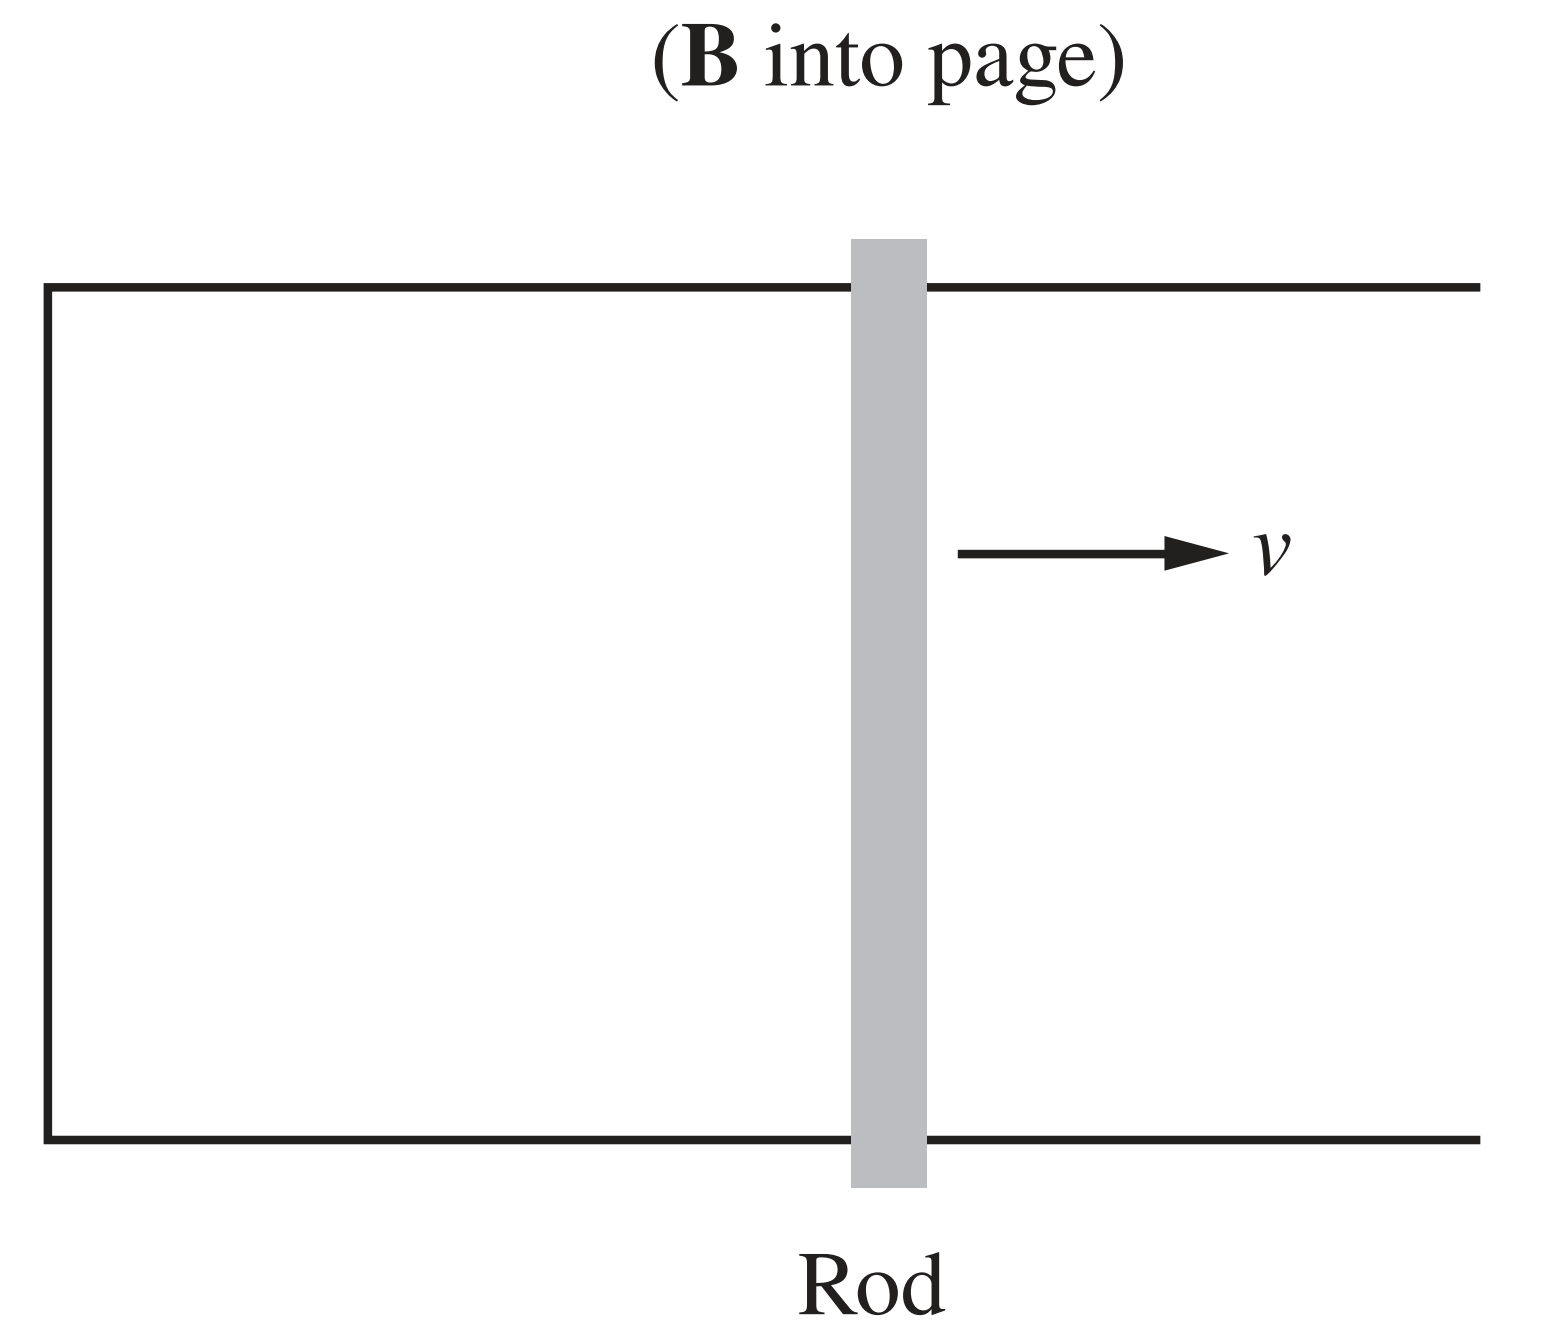
\includegraphics[width=5cm]{rod_slide.png}
\end{center}
\end{prob}

\begin{sol}
    We know the magnetic field can never do work because it always points perpendicular to the velocity. So, the answer is just that it is you / whoever is pulling the rod that is doing work. The charges inside of the rod are both moving rightward and upward, so  there is a nonzero rightward component which is parallel to the force you apply on the rod, leading to you doing work.
\end{sol}


\begin{prob}[Purcell]
    An infinite solenoid with radius $b$ has $n$ turns per unit length. The current varies in time according to $I(t) = I_0 \cos \omega t$ (with positive defined as shown below). A ring with radius $r < b$ and resistance $R$ is centered on the solenoid's axis, with its plane perpendicular to the axis.
    \begin{center}
        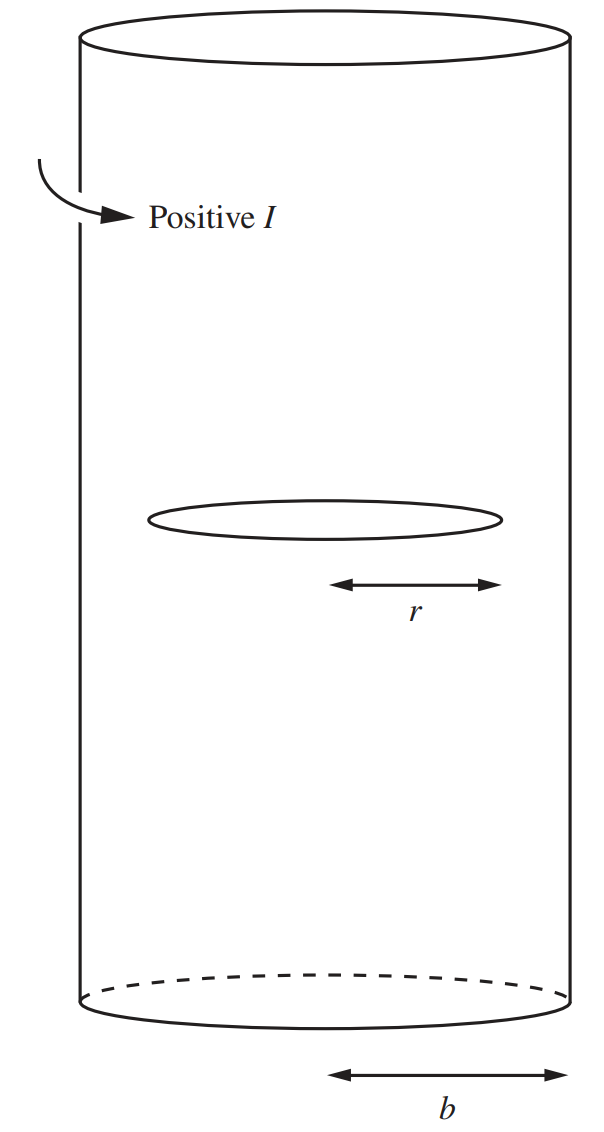
\includegraphics[width=4cm]{ring_flip.png}
    \end{center}
    \begin{anum}
        \item What is the induced current in the ring?
        \item A given little piece of the ring will feel a magnetic force. For what values of $t$ is this force maximum?
        \item What is the effect of the force on the ring? That is, does the force cause the ring to translate, spin, flip over, stretch/shrink, etc.?
    \end{anum}
\end{prob}
\begin{alphasol}
    \item The magnetic field generated by the solenoid is $B(t) = \mu_0 n I(t)$, so $\Phi_B (t) = \mu_0 n\pi r^2 I(t)$. So, by Faraday's law,
    $$\mathcal E = \left |\frac{d \Phi_B}{dt}\right| = \mu_0 n \pi r^2 I_0\omega \sin \omega t.$$
    Thus, the induced current is $i(t) = \mathcal E/R = \frac{\mu_0 n \pi \omega r^2 I_0}{R}\sin \omega t.$
    \item The force is given by $F = i l B$ and since $i \propto \sin \omega t$ and $B \propto \cos \omega t$, so
    $$F \propto \sin \omega t \cos \omega t = \sin (2\omega t),$$
    which means it is maximum when $\omega t = \pi / 4 + k\pi /2$ where $k \in \mathbb Z$.
    \item The effect is to stretch/shrink the ring, by Lenz's law and right hand rule.
\end{alphasol}


\begin{prob}[PPP]
    A homogeneous field of magnetic induction $\mathbf B$ is perpendicular to a track of width $\ell$ which is inclined at an angle $\alpha$ to the horizontal. A frictionless conducting rod of mass $m$ straddles the two rails of the track as shown in the figure below.
    \begin{center}
        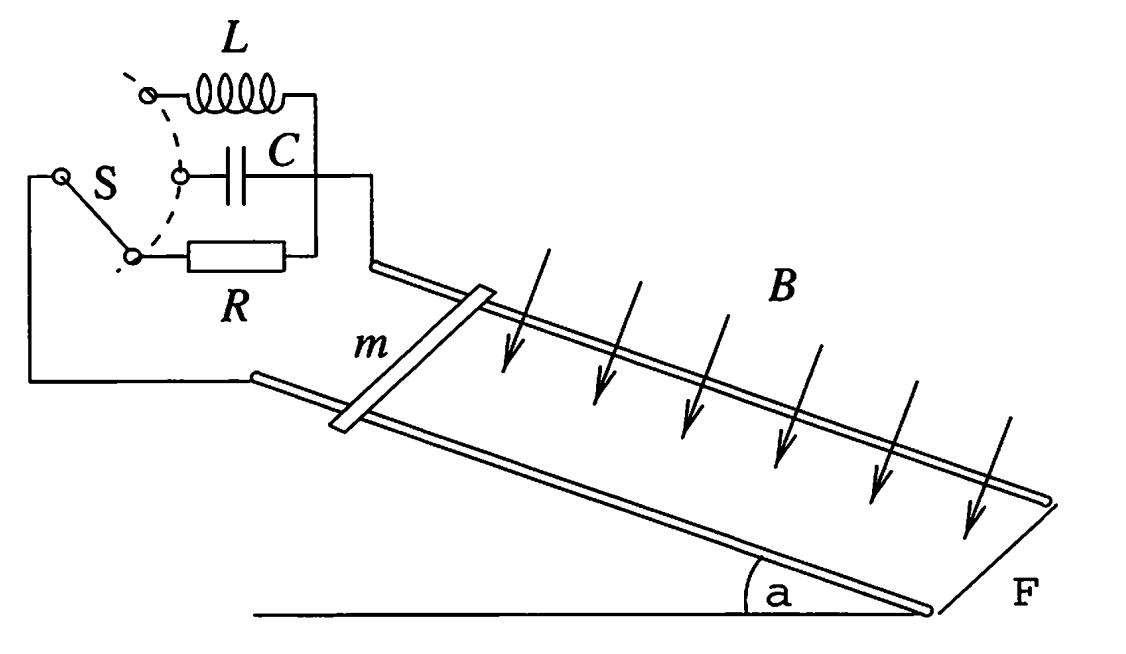
\includegraphics[width=6cm]{track_slide.png}
    \end{center}
    How does the rod move, after being released from rest, if the circuit formed by the rod and the track is closed by:
    \begin{anum}
        \item a resistor of resistance $R$,
        \item a capacitor of capacitance $C$, or
        \item a coil of inductance $L$?
    \end{anum}
\end{prob}
\begin{alphasol}
    \item We saw almost the same problem in lecture. We again want to write a differential equation. On the rod we can write $F=ma$:
    $$ma = mg \sin \alpha - I \ell B,$$
    and we can also write Kirchoff's loop rule:
    $$IR = \mathcal E = v B \ell.$$
    And so we can replace $I$ in the first equation, giving us
    $$\frac{dv}{dt} = g\sin \alpha - v\frac{\ell^2 B^2}{mR},$$
    which tells us that the rod exponentially decays to a terminal velocity of $\frac{mg R \sin \alpha}{B^2 \ell^2}$.
    \item The $F=ma$ equation is the same in this case, but we now have
    $$\frac QC = v B \ell.$$
    Thus, differentiating and putting into the $F=ma$ equation, we get
    $$\frac{dv}{dt} = g\sin \alpha - \frac{B^2 \ell^2 C}{m} \frac{dv}{dt},$$
    which tells us that $dv/dt = \frac{g\sin \alpha}{1 + B^2\ell^2 C/m}$. Thus, the rod slides down with constant acceleration.
    \item Lastly, with the case of an inductor, we have
    $$vB \ell = L\frac{dI}{dt},$$
    and differentiating the $F=ma$ equation, we get
    $$\frac{d^2 v}{dt^2} = - \ell B \frac{vB\ell}{L} = -\frac{\ell^2 B^2}{L} v,$$
    which is simple harmonic motion.
\end{alphasol}

\begin{prob}\label{nrg_prob}
    Show that the energy stored in two inductors of inductances $L_1,L_2$ and mutual inductance $M$ is given by,
    $$U(I_1,I_2) = \frac 12 L_1 I_1^2 + \frac 12 L_2 I_2^2 + MI_1I_2.$$
    \textit{Hint:} imagine ``charging up'' one inductor first and then the next one.
\end{prob}
\begin{sol}
    Based on the definition of inductance, we have the following differential,
    $$dU = (L_1I_1 + MI_2)dI_1 + (L_2I_2 +MI_1)dI_2.$$
    Integrating in order,
    $$U(I_1,0) =\int_0^{I_1} L_1I_1\, dI_1 =  \frac 12 L_1 I_1^2.$$
    And
    $$U(I_1,0) = \frac 12 L_1 I_1^2 + \int_0^{I_2} L_2 I_2 + MI_1 \, dI_2 =\frac 12 L_1 I_1^2 + \frac 12 L_2 I_2^2 + MI_1I_2,$$
    as desired.
\end{sol}


\begin{prob}
    Suppose you have two identical solenoids of radii $r$, length $l$, and $N$ turns separated by a distance $d \gg l \gg r$.
    \begin{anum}
        \item Suppose their axes are aligned as shown below. What is their mutual inductance?
        \begin{center}
            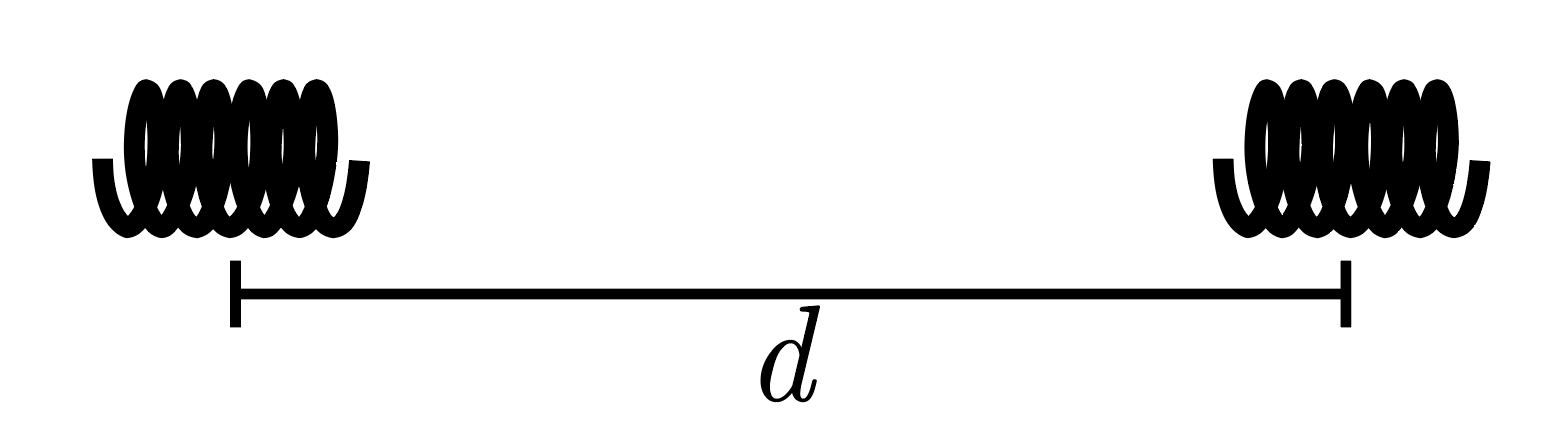
\includegraphics[width=5cm]{alig_mut.png}
        \end{center}
        \item Suppose they are now aligned perpendicular to each other as shown below. What is their mutual inductance?
        \begin{center}
            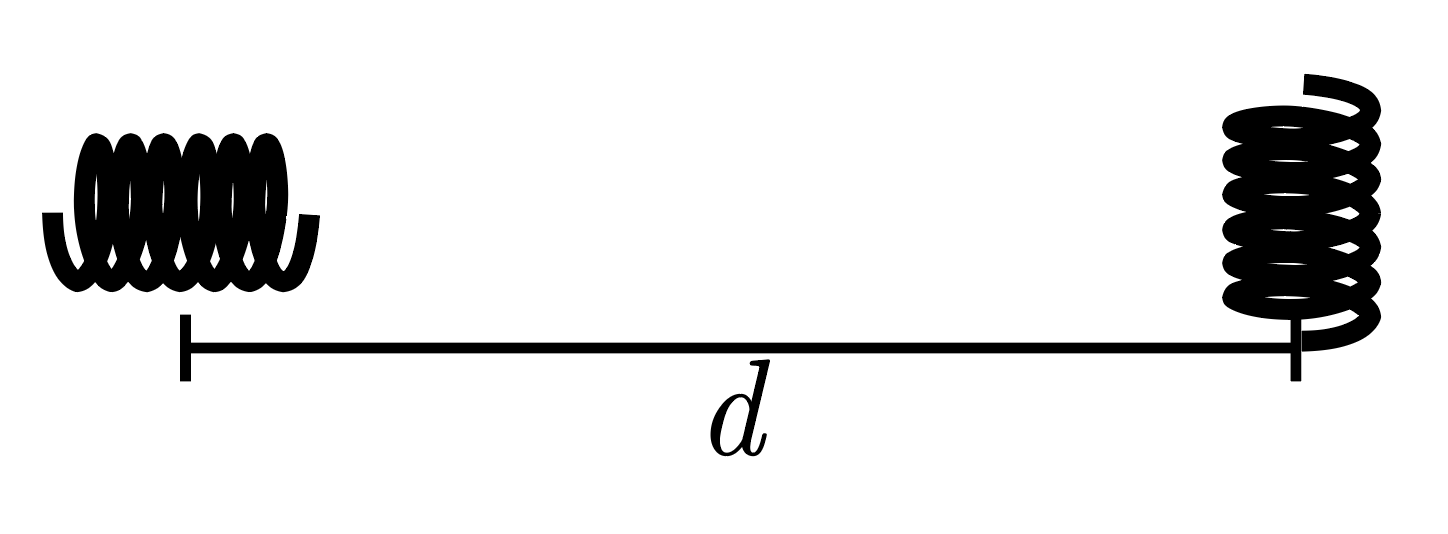
\includegraphics[width=5cm]{perp_mut.png}
        \end{center}
        \item Using the result from problem \ref{nrg_prob}, find the force between the solenoids in each case if a current $I$ is maintained on each solenoid.
    \end{anum}
\end{prob}
\begin{alphasol}
    \item A solenoid from far away is effectively a magnetic dipole with magnetic moment
    $$m = N (\pi r^2) I.$$
    Thus, the field at a distance $d \gg r$ along the axis of a magnetic dipole is
    $$B = \frac{\mu_0 m}{2\pi d^3} = \frac{\mu_0 N r^2 I}{2d^3}.$$
    Thus, flux due to one solenoid on the other is 
    $$\Phi = \frac{\mu_0 N^2 \pi r^4 I}{2 d^3},$$
    which means that the mutual inductance is $M = \frac{\mu_0 \pi N^2 r^4}{2d^3}.$
    \item This time we consider the flux through the left solenoid due to the right solenoid. So, to first order, the mutual inductance is $0$.
    \item For part (b) becaus there is no mutual inductance -- no interaction -- the force is immediately 0. For part (a), we can write out the interaction energy and take a derivative w.r.t to distance:
    $$U(d) = MI_1I_2 = \frac{\mu_0 \pi N^2 r^4 I^2}{2d^3}.$$
    Thus, the force is
    $$F = -\frac{dU}{dd} = -\frac{3\mu_0 \pi N^2 r^4 I^2}{2d^4}.$$
This matches the dipole formula for force $\mathbf F = \nabla (\mathbf m \cdot \mathbf B).$
\end{alphasol}


\begin{prob}
    In class, we discussed the falling of a magnet through a metal tube. In this problem, we estimate the terminal speed of the magnet. A magnet of magnetic moment $\mu$, mass $m$, and characteristic size $a$ falls through a metal tube of radius $R$, thickness $d$ and resistivity $\rho$ with speed $v$. \begin{anum}
        \item Using physical reasoning and dimensional analysis, estimate the force on the magnet from the tube.
        \item Finish by determining the terminal speed of the magnet.
    \end{anum}
\end{prob}
\begin{alphasol}
    \item We can first estimate the rate of change of magnetic flux due to the magnet as
    $$\frac{d\Phi_B}{dt} \sim BR^2 \frac{v}{a} = \frac{\mu_0 \mu}{R^3} R^2 \frac va.$$
    Now, the resistance of the relevant section of the cylinder is $R \sim \rho R/(dR) \sim \rho/d$, so the current in the cylinder is
    $$I \sim \frac{\mu_0 \mu v d}{\rho R a}.$$
    Now, by biot-savart's law the magnetic field in the center of the cylinder is on the order of $\mu_0 I R/R^2 \sim \mu_0 I/R$, and using the formula for the force on a dipole due to a change magnetic field, we can estimate
    $$F \sim \frac{\mu_0 I/R}{R} \mu \frac{d}{a} = \frac{(\mu_0 \mu)^2 v d}{\rho R^3a}.$$
    \item We just set the force equal to $mg$ now and we get $$v \sim \frac{mg \rho R^3 a}{(\mu_0 \mu)^2 d}.$$
\end{alphasol}

%https://www.ioc.ee/~kalda/ipho/es/e-s-2015-eng.pdf
\begin{prob}[EFPhO]
    We worked with solenoids far away from each other, but now we deal with two that are right next to each other. You have two solenoids, each with $N$ turns, length $l$, and cross sectional areas $A_1 < A_2 \ll l^2$. They are each connected to a constant current source of magnitude $I$ and then the smaller solenoid is placed inside the other one such that the centers of the solenoids are a distance $x < l$ apart.
    \begin{anum}
        \item Assuming that $A_1,A_2 \ll x^2, (l-x)^2$, find the total energy $E_m$ of the magnetic fields in this system.
        \item Find the electromotive forces
        $\mathcal E_1$ and $\mathcal E_2$ generated on the coils when one is
        pulled out with a speed $v$.
        \item Find the force $F$ needed to pull
        one coil outwards.
    \end{anum}
\end{prob}
\begin{sol}
    \officialsol{https://www.ioc.ee/~kalda/ipho/es/e-s-2015-sol.pdf\#page=3}
\end{sol}

\begin{prob}
    A charge of charge $q$ and mass $m$ is orbiting in a circle of radius $r$ due to a uniform magnetic field of magnitude $B$. If the magnitude of the magnetic field is slowly increased to $2B$ -- slow enough such that the charge remains in an approximately circular orbit -- what is the final radius of the charge's orbit?
\end{prob}

\begin{sol}
    By faraday's law, we have that
    $$\oint \mathbf E \cdot d \mathbf r = -\frac{d \Phi_B}{d t} = -\pi r^2 \frac{dB}{dt}.$$
    Thus, in an orbit, we have the rate of change of kinetic energy of the mass is
    $$\frac{dK}{dt} = qEv = q\frac{\pi r^2}{2\pi r} \frac{dB}{dt}v,$$
    where it is positive by Lenz's law. Plugging in the kinetic energy term, it become s
    $$mv \frac{dv}{dt} = \frac{qvr}{2} \frac{dB}{dt}.$$
    From the standard lorentz force, we also have
    $$qvB = \frac{mv^2}{r} \implies v = \frac{qBr}{m}.$$
    Plugging this into the differential equation, we get
    $$qBr \frac{qB}{m}\frac{dr}{dt} + qBr\frac{qr}{m}\frac{dB}{dt} = \frac{q^2Br^2}{2m}\frac{dB}{dt}.$$
    Simplifying and integrating both sides with respect to time,
    $$\int_{r}^{r_f} \frac 1r \, dr = -\frac 12 \int_{B}^{2B} \frac 1B \, dB \implies \ln(r_f/r) = -\frac 12 \ln (2) \implies r_f =  r/\sqrt 2.$$
\end{sol}


\subsection{Challenge Problems}

%that one usapho+ problem about axions

\begin{prob}
    \href{https://www.aapt.org/physicsteam/upload/2023-USAPhO-Exam.pdf\#page=9}{2023 USAPhO, B1}
\end{prob}
\begin{sol}
    \officialsol{https://www.aapt.org/physicsteam/2023/upload/2023-USAPhO-solutions.pdf\#page=15}
\end{sol}

\begin{prob}
    \href{https://apho.olimpicos.net/pdf/APhO_2009_Q2.pdf}{2009 APhO, T2}
\end{prob}
\begin{sol}
    \officialsol{https://apho.olimpicos.net/pdf/APhO_2009_S2.pdf}
\end{sol}

\begin{prob}
    \href{https://apho.olimpicos.net/pdf/APhO_2011_Q1.pdf}{2011 APhO, T1}
\end{prob}
\begin{sol}
    \officialsol{https://apho.olimpicos.net/pdf/APhO_2011_S1.pdf}
\end{sol}



\subsection{USAPhO Practice}

%USAPhO 2020/A1
\begin{prob}[USAPhO 2020 A1]
    An infinitely long wire with linear charge density $-\lambda$ lies along the $z$-axis. An infinitely long insulating cylindrical shell of radius $a$ is concentric with the wire and can rotate freely about the $z$-axis. The shell has moment of inertia per unit length $I$. Charge is uniformly distributed on the shell, with surface charge density $\frac{\lambda}{2\pi a}$.

    The system is immersed in an external magnetic field $B_0\hat{\mathbf z}$, and is initially at rest. Starting at $t = 0$, the external magnetic field is slowly reduced to zero over a time $T \gg a/c$, where $c$ is the speed of light.
    \begin{center}
        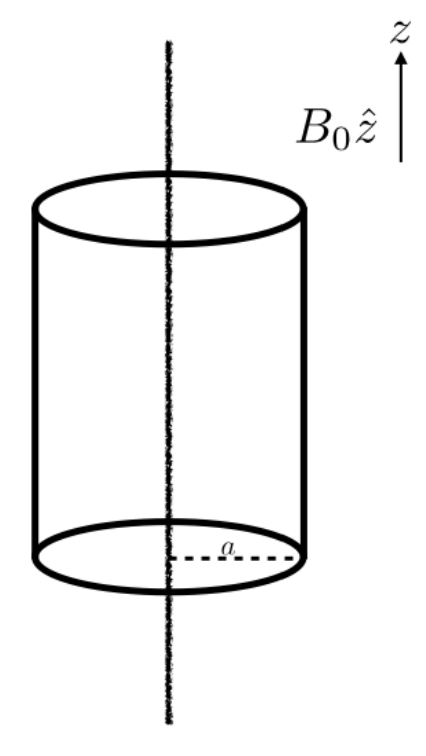
\includegraphics[width=3cm]{2020usaphoa1.png}
    \end{center}

    \begin{anum}
        \item Find an expression of the final angular velocity $\omega$ of the cylinder in terms of the symbols given
        and other constants.
        \item You may be surprised that the expression you find above is not zero! However, the electric and
        magnetic fields can have angular momentum. Analogous to the ``regular'' angular momentum
        definition, the EM field angular momentum per unit volume at a displacement $\mathbf r$ from the axis
        of rotation is:
        $$\mathcal L (\mathbf r) = \mathbf r \times \mathcal P (\mathbf r).$$
        $\mathcal P(\mathbf r)$ is a vector analogous to momentum, given by
        $$\mathcal P (\mathbf r) = \alpha \cdot (\mathbf E (\mathbf r) \times \mathbf B (\mathbf r)),$$
        where $\alpha$ is some proportionality constant. Find an expression for $\alpha$ in terms of given variables and fundamental constants.
    \end{anum}
\end{prob}
\begin{sol}
    \officialsol{https://www.aapt.org/Common/upload/2020_USAPhO_solutions.pdf} There may be some typos in the official solutions though, so ask questions if you have them.
\end{sol}

\begin{prob}
    Magnetic braking is a contactless braking system which uses electromagnetic induction and magnetic interactions to its advantage. We begin by exploring simpler scenarios involving conductors and magnetic fields.
    \begin{anum}
        \item First, suppose we have a conducting cylinder with radius $R$ and length $L \gg R$. It is placed inside a uniform magnetic field with magnitude $B$ and direction parallel to its axis and rotates at constant angular velocity $\omega$. After a long time, find the charge distribution on the conducting cylinder.
        \begin{center}
            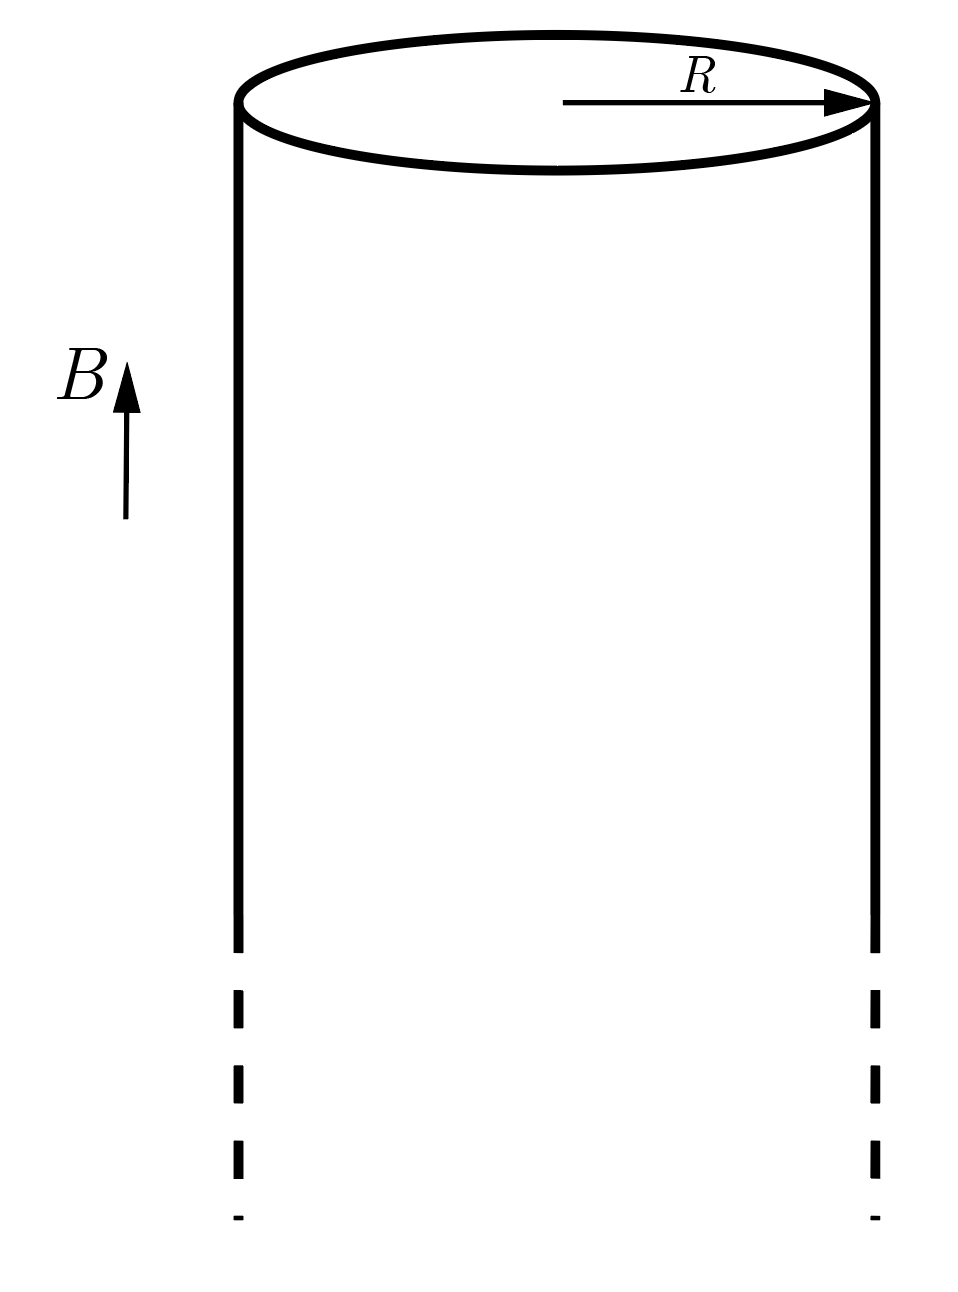
\includegraphics[width=5cm]{cylin_brake.png}
        \end{center}
        \item Now, we replace the cylinder with a disk of radius $R$ and attach a current source of magnitude $I$ to the center and outer radius of the disk as shown below. What is the torque that is applied to the disk due to the magnetic field?
        \begin{center}
            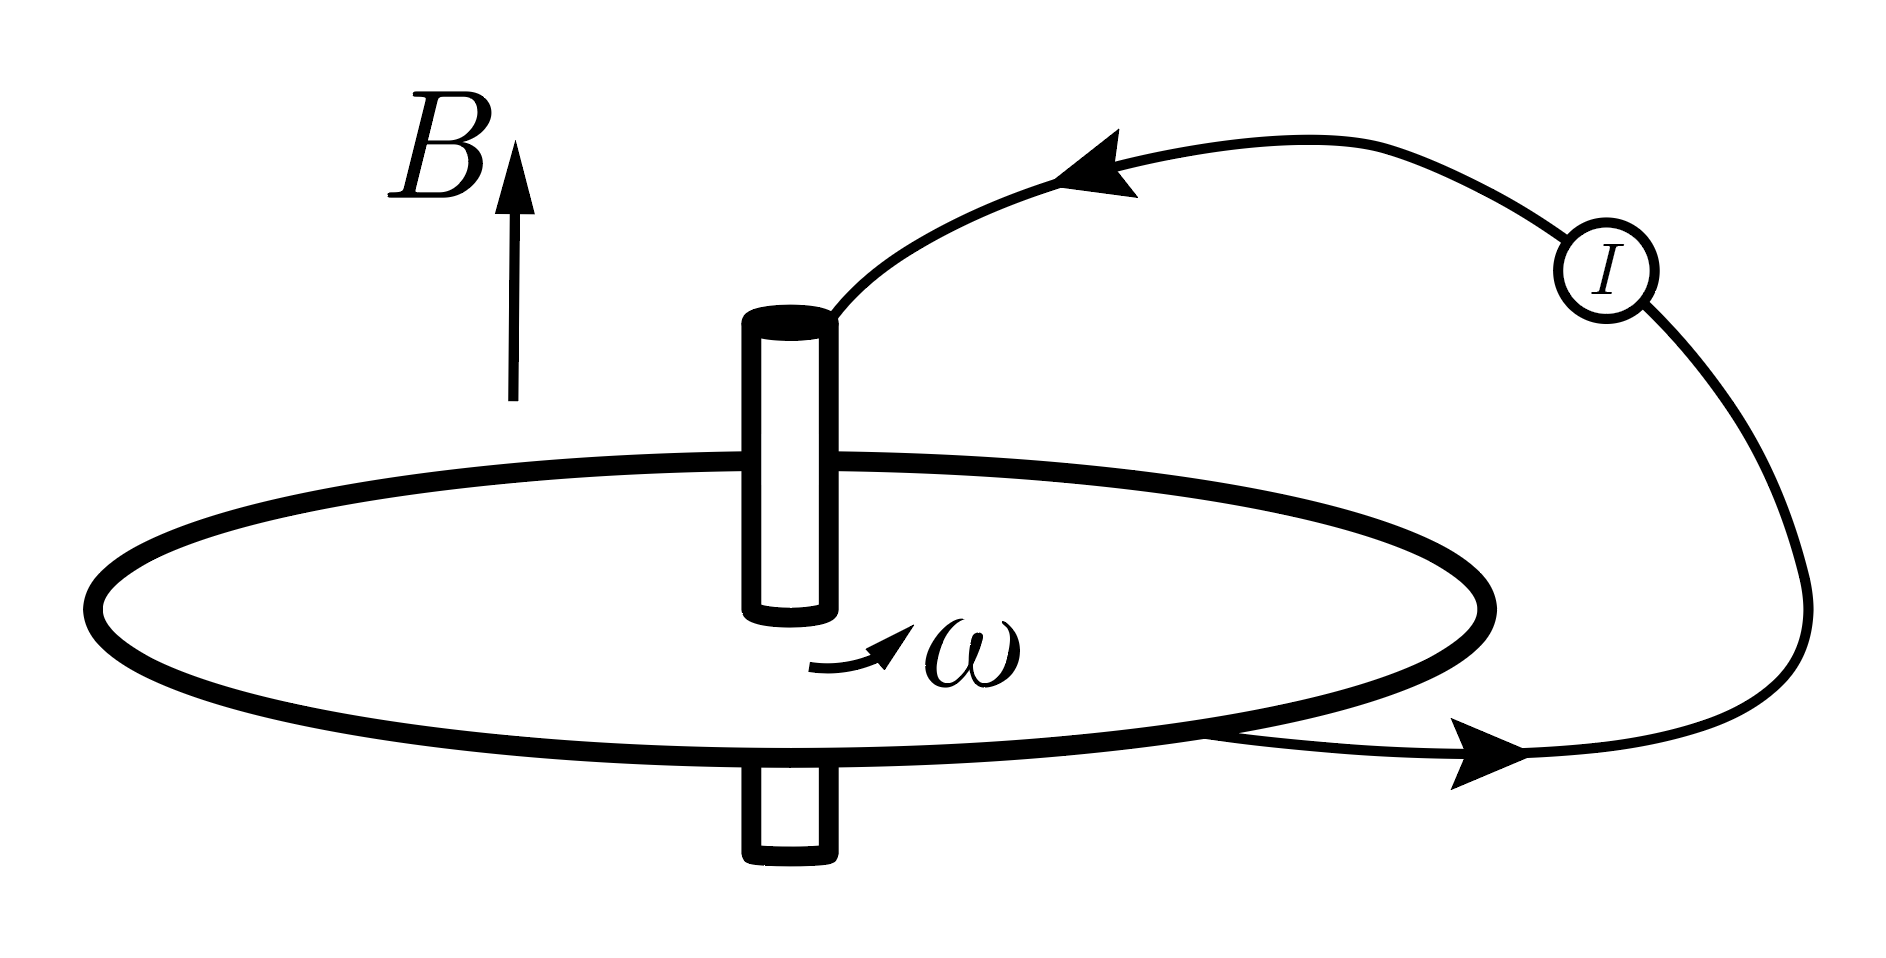
\includegraphics[width=6.5cm]{spin_brake.png}
        \end{center}
        \item What is the EMF applied by the current source as a function of time in order to maintain the constant current $I$?
        \item In magnetic braking, the magnetic field is only applied to a small portion of the disk. Suppose that it is applied on some sector of size $\theta$ as shown below. Furthermore, assume for ease that the disk is actually produced of many radial wires as shown below. What is the braking torque experienced by the disk? Also assume for ease that each ``triangle'' in the disk can only flow current within its own loop and has total resistance $R_{\text{triangle}}.$
        \begin{center}
            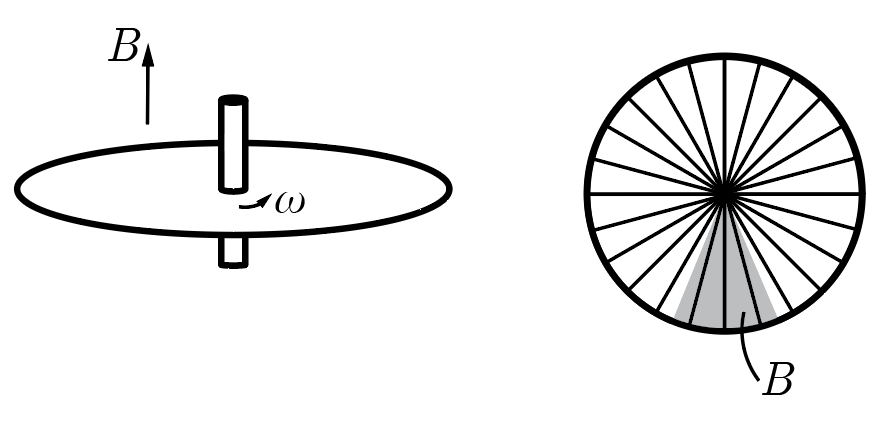
\includegraphics[width=8cm]{spoke_brake.png}
        \end{center}
    \end{anum}
\end{prob}
\begin{alphasol}
    \item After a long time, in the rotating frame, the net force on particles with charge $q$ within the cylinder should be 0. The force field due to the magnetic force at a radius $r$ is $\omega r B$. Thus, we can write
    $$qE + q\omega r B = m \omega^2 r \implies E(r) = (m\omega^2/q - \omega B) r.$$
    Suppose that at a radius $r$ we have charge enclose $Q$. Then, by Gauss's law, we have
    $$2\pi r \ell E(r) = \frac{Q}{\epsilon_0} \implies Q(r) = 2\pi\epsilon_0 r^2 \ell  (m \omega ^2/q - \omega B) .$$
    if we want to have a charge distribution that is proportional to $r^2$ since the integral for charge is
    $$Q = \int \rho (2\pi r\ell)\, dr,$$
    we get an $r^2$ proportionality if $\rho$ is constant. Thus, we have
    $$Q(r) = \rho \pi r^2 \ell \implies \rho = 2\epsilon_0 (m\omega^2/q - \omega B).$$
    \item Consider a total current $I$ flowing from radius $r$ to radius $r + dr$. We have that the torque is equal to
    $$d\tau = r\cdot (I (dr) B),$$
    so the total torque is
    $$\tau = \int_0^R d\tau = \int_0^R IB r\, dr =\boxed{ \frac 12 IBR^2}.$$
    \item The emf generated by the magnetic force at a radius $r$ is equal to
    $$\mathcal E = \int_0^R \omega r B\, dr = \frac 12 \omega BR^2. $$
    \item Consider a small triangular sector that is going through the transition region. The rate of change of flux is
    $$\frac{d\Phi_B}{dt} = B \frac{dA}{dt} = -B \frac 12 R^2 \frac{d\theta}{dt} = -\frac{B\omega R^2}{2},$$
    which is the same expression as part (c) (can you explain why?). So, the current through a loop is
    $$I = \frac{B\omega R^2}{2R_{\text{triangle}}}.$$
    Now, using the same strategy as part (b), we have that the torque on the wire that is in the magnetic field is
    $$\tau = \int_0^R IB r \, dr = \frac 12 IBR^2.$$
    But there are two total triangles going through transition regions, so the total braking torque is
    $$2 \tau = IBR^2 = \frac{B^2 \omega R^4}{2R_{\text{triangle}}}.$$
\end{alphasol}



\end{document}